% Options for packages loaded elsewhere
\PassOptionsToPackage{unicode}{hyperref}
\PassOptionsToPackage{hyphens}{url}
%
\documentclass[
]{article}
\usepackage{amsmath,amssymb}
\usepackage{iftex}
\ifPDFTeX
  \usepackage[T1]{fontenc}
  \usepackage[utf8]{inputenc}
  \usepackage{textcomp} % provide euro and other symbols
\else % if luatex or xetex
  \usepackage{unicode-math} % this also loads fontspec
  \defaultfontfeatures{Scale=MatchLowercase}
  \defaultfontfeatures[\rmfamily]{Ligatures=TeX,Scale=1}
\fi
\usepackage{lmodern}
\ifPDFTeX\else
  % xetex/luatex font selection
\fi
% Use upquote if available, for straight quotes in verbatim environments
\IfFileExists{upquote.sty}{\usepackage{upquote}}{}
\IfFileExists{microtype.sty}{% use microtype if available
  \usepackage[]{microtype}
  \UseMicrotypeSet[protrusion]{basicmath} % disable protrusion for tt fonts
}{}
\makeatletter
\@ifundefined{KOMAClassName}{% if non-KOMA class
  \IfFileExists{parskip.sty}{%
    \usepackage{parskip}
  }{% else
    \setlength{\parindent}{0pt}
    \setlength{\parskip}{6pt plus 2pt minus 1pt}}
}{% if KOMA class
  \KOMAoptions{parskip=half}}
\makeatother
\usepackage{xcolor}
\usepackage[margin=1in]{geometry}
\usepackage{color}
\usepackage{fancyvrb}
\newcommand{\VerbBar}{|}
\newcommand{\VERB}{\Verb[commandchars=\\\{\}]}
\DefineVerbatimEnvironment{Highlighting}{Verbatim}{commandchars=\\\{\}}
% Add ',fontsize=\small' for more characters per line
\usepackage{framed}
\definecolor{shadecolor}{RGB}{248,248,248}
\newenvironment{Shaded}{\begin{snugshade}}{\end{snugshade}}
\newcommand{\AlertTok}[1]{\textcolor[rgb]{0.94,0.16,0.16}{#1}}
\newcommand{\AnnotationTok}[1]{\textcolor[rgb]{0.56,0.35,0.01}{\textbf{\textit{#1}}}}
\newcommand{\AttributeTok}[1]{\textcolor[rgb]{0.13,0.29,0.53}{#1}}
\newcommand{\BaseNTok}[1]{\textcolor[rgb]{0.00,0.00,0.81}{#1}}
\newcommand{\BuiltInTok}[1]{#1}
\newcommand{\CharTok}[1]{\textcolor[rgb]{0.31,0.60,0.02}{#1}}
\newcommand{\CommentTok}[1]{\textcolor[rgb]{0.56,0.35,0.01}{\textit{#1}}}
\newcommand{\CommentVarTok}[1]{\textcolor[rgb]{0.56,0.35,0.01}{\textbf{\textit{#1}}}}
\newcommand{\ConstantTok}[1]{\textcolor[rgb]{0.56,0.35,0.01}{#1}}
\newcommand{\ControlFlowTok}[1]{\textcolor[rgb]{0.13,0.29,0.53}{\textbf{#1}}}
\newcommand{\DataTypeTok}[1]{\textcolor[rgb]{0.13,0.29,0.53}{#1}}
\newcommand{\DecValTok}[1]{\textcolor[rgb]{0.00,0.00,0.81}{#1}}
\newcommand{\DocumentationTok}[1]{\textcolor[rgb]{0.56,0.35,0.01}{\textbf{\textit{#1}}}}
\newcommand{\ErrorTok}[1]{\textcolor[rgb]{0.64,0.00,0.00}{\textbf{#1}}}
\newcommand{\ExtensionTok}[1]{#1}
\newcommand{\FloatTok}[1]{\textcolor[rgb]{0.00,0.00,0.81}{#1}}
\newcommand{\FunctionTok}[1]{\textcolor[rgb]{0.13,0.29,0.53}{\textbf{#1}}}
\newcommand{\ImportTok}[1]{#1}
\newcommand{\InformationTok}[1]{\textcolor[rgb]{0.56,0.35,0.01}{\textbf{\textit{#1}}}}
\newcommand{\KeywordTok}[1]{\textcolor[rgb]{0.13,0.29,0.53}{\textbf{#1}}}
\newcommand{\NormalTok}[1]{#1}
\newcommand{\OperatorTok}[1]{\textcolor[rgb]{0.81,0.36,0.00}{\textbf{#1}}}
\newcommand{\OtherTok}[1]{\textcolor[rgb]{0.56,0.35,0.01}{#1}}
\newcommand{\PreprocessorTok}[1]{\textcolor[rgb]{0.56,0.35,0.01}{\textit{#1}}}
\newcommand{\RegionMarkerTok}[1]{#1}
\newcommand{\SpecialCharTok}[1]{\textcolor[rgb]{0.81,0.36,0.00}{\textbf{#1}}}
\newcommand{\SpecialStringTok}[1]{\textcolor[rgb]{0.31,0.60,0.02}{#1}}
\newcommand{\StringTok}[1]{\textcolor[rgb]{0.31,0.60,0.02}{#1}}
\newcommand{\VariableTok}[1]{\textcolor[rgb]{0.00,0.00,0.00}{#1}}
\newcommand{\VerbatimStringTok}[1]{\textcolor[rgb]{0.31,0.60,0.02}{#1}}
\newcommand{\WarningTok}[1]{\textcolor[rgb]{0.56,0.35,0.01}{\textbf{\textit{#1}}}}
\usepackage{graphicx}
\makeatletter
\newsavebox\pandoc@box
\newcommand*\pandocbounded[1]{% scales image to fit in text height/width
  \sbox\pandoc@box{#1}%
  \Gscale@div\@tempa{\textheight}{\dimexpr\ht\pandoc@box+\dp\pandoc@box\relax}%
  \Gscale@div\@tempb{\linewidth}{\wd\pandoc@box}%
  \ifdim\@tempb\p@<\@tempa\p@\let\@tempa\@tempb\fi% select the smaller of both
  \ifdim\@tempa\p@<\p@\scalebox{\@tempa}{\usebox\pandoc@box}%
  \else\usebox{\pandoc@box}%
  \fi%
}
% Set default figure placement to htbp
\def\fps@figure{htbp}
\makeatother
\setlength{\emergencystretch}{3em} % prevent overfull lines
\providecommand{\tightlist}{%
  \setlength{\itemsep}{0pt}\setlength{\parskip}{0pt}}
\setcounter{secnumdepth}{-\maxdimen} % remove section numbering
\usepackage{bookmark}
\IfFileExists{xurl.sty}{\usepackage{xurl}}{} % add URL line breaks if available
\urlstyle{same}
\hypersetup{
  pdftitle={Aula6 - Visualização de dados},
  hidelinks,
  pdfcreator={LaTeX via pandoc}}

\title{Aula6 - Visualização de dados}
\author{}
\date{\vspace{-2.5em}2025-02-13}

\begin{document}
\maketitle

\subsection{Importando bibliotecas para
análise}\label{importando-bibliotecas-para-anuxe1lise}

\begin{Shaded}
\begin{Highlighting}[]
\FunctionTok{library}\NormalTok{(tidyverse)}
\end{Highlighting}
\end{Shaded}

\begin{verbatim}
## -- Attaching core tidyverse packages ------------------------ tidyverse 2.0.0 --
## v dplyr     1.1.4     v readr     2.1.5
## v forcats   1.0.0     v stringr   1.5.1
## v ggplot2   3.5.1     v tibble    3.2.1
## v lubridate 1.9.4     v tidyr     1.3.1
## v purrr     1.0.4     
## -- Conflicts ------------------------------------------ tidyverse_conflicts() --
## x dplyr::filter() masks stats::filter()
## x dplyr::lag()    masks stats::lag()
## i Use the conflicted package (<http://conflicted.r-lib.org/>) to force all conflicts to become errors
\end{verbatim}

\begin{Shaded}
\begin{Highlighting}[]
\FunctionTok{library}\NormalTok{(readxl)}
\FunctionTok{library}\NormalTok{(knitr)}
\FunctionTok{library}\NormalTok{(data.table)}
\end{Highlighting}
\end{Shaded}

\begin{verbatim}
## 
## Attaching package: 'data.table'
## 
## The following objects are masked from 'package:lubridate':
## 
##     hour, isoweek, mday, minute, month, quarter, second, wday, week,
##     yday, year
## 
## The following objects are masked from 'package:dplyr':
## 
##     between, first, last
## 
## The following object is masked from 'package:purrr':
## 
##     transpose
\end{verbatim}

\subsection{Importando os dados}\label{importando-os-dados}

Vamos importar os dados de crimes ocorridos e registrados pelos
batalhões do estado do Rio de Janeiro.

\begin{Shaded}
\begin{Highlighting}[]
\NormalTok{crimes }\OtherTok{\textless{}{-}}\NormalTok{ readr}\SpecialCharTok{::}\FunctionTok{read\_csv2}\NormalTok{(}\StringTok{"/Users/ottotavares/Library/Mobile Documents/com\textasciitilde{}apple\textasciitilde{}CloudDocs/Documents/infnet/Estatistica\_Ciencia\_Dados\_2024/dados\_auxiliares/BaseDPEvolucaoMensalCisp.csv"}\NormalTok{, }\AttributeTok{locale =}\NormalTok{ readr}\SpecialCharTok{::}\FunctionTok{locale}\NormalTok{(}\AttributeTok{encoding =} \StringTok{"latin1"}\NormalTok{))}
\end{Highlighting}
\end{Shaded}

\begin{verbatim}
## i Using "','" as decimal and "'.'" as grouping mark. Use `read_delim()` for more control.
\end{verbatim}

\begin{verbatim}
## Rows: 32245 Columns: 63
## -- Column specification --------------------------------------------------------
## Delimiter: ";"
## chr  (3): mes_ano, munic, Regiao
## dbl (60): CISP, mes, ano, AISP, RISP, mcirc, hom_doloso, lesao_corp_morte, l...
## 
## i Use `spec()` to retrieve the full column specification for this data.
## i Specify the column types or set `show_col_types = FALSE` to quiet this message.
\end{verbatim}

\subsection{Limpando as datas e selecionando as variáveis de
interesse}\label{limpando-as-datas-e-selecionando-as-variuxe1veis-de-interesse}

\begin{Shaded}
\begin{Highlighting}[]
\CommentTok{\#Ajustando as datas, selecionando variáveis de interesse}
\CommentTok{\#crimes$mes.ano \textless{}{-} as.IDate(paste("01", unlist(lapply(strsplit(crimes$mes\_ano, split = "m"), function(x) x[2])), unlist(lapply(strsplit(crimes$mes\_ano, split = "m"), function(x) x[1])), sep = "{-}"), format = "\%d{-}\%m{-}\%Y")}

\NormalTok{crimes }\OtherTok{\textless{}{-}}\NormalTok{ crimes }\SpecialCharTok{\%\textgreater{}\%}\NormalTok{ dplyr}\SpecialCharTok{::}\FunctionTok{mutate}\NormalTok{(}\AttributeTok{mes.ano =} \FunctionTok{as.IDate}\NormalTok{(}\FunctionTok{paste}\NormalTok{(}\StringTok{"01"}\NormalTok{, mes, ano, }\AttributeTok{sep =} \StringTok{"{-}"}\NormalTok{), }\AttributeTok{format =} \StringTok{"\%d{-}\%m{-}\%Y"}\NormalTok{)) }\SpecialCharTok{\%\textgreater{}\%}\NormalTok{ dplyr}\SpecialCharTok{::}\FunctionTok{select}\NormalTok{(CISP, mes.ano, AISP, roubo\_cx\_eletronico}\SpecialCharTok{:}\NormalTok{apreensao\_drogas\_sem\_autor)}



\CommentTok{\#Filtrando apenas para as regi˜}
\end{Highlighting}
\end{Shaded}

\#Agregando variáveis por batalhão para facilitar a visualização e
selecionando apenas três batalhões de interesse

\begin{Shaded}
\begin{Highlighting}[]
\NormalTok{crimes.regioes }\OtherTok{\textless{}{-}}\NormalTok{ crimes }\SpecialCharTok{\%\textgreater{}\%}\NormalTok{ dplyr}\SpecialCharTok{::}\FunctionTok{group\_by}\NormalTok{(AISP, mes.ano) }\SpecialCharTok{\%\textgreater{}\%}\NormalTok{ dplyr}\SpecialCharTok{::}\FunctionTok{summarise\_at}\NormalTok{(}\FunctionTok{vars}\NormalTok{(furto\_veiculos}\SpecialCharTok{:}\NormalTok{total\_furtos), sum)}

\CommentTok{\#Dando nome aos bairros atendidos pelos batalhões em questão e em seguida os selecionando como batalhões de interesse}

\NormalTok{crimes.regioes}\SpecialCharTok{$}\NormalTok{aisp.nm }\OtherTok{\textless{}{-}} \FunctionTok{ifelse}\NormalTok{(crimes.regioes}\SpecialCharTok{$}\NormalTok{AISP }\SpecialCharTok{==} \DecValTok{2}\NormalTok{, }\StringTok{"Botafogo"}\NormalTok{, }\FunctionTok{ifelse}\NormalTok{(crimes.regioes}\SpecialCharTok{$}\NormalTok{AISP }\SpecialCharTok{==} \DecValTok{26}\NormalTok{, }\StringTok{"Teresópolis"}\NormalTok{,  }\FunctionTok{ifelse}\NormalTok{(crimes.regioes}\SpecialCharTok{$}\NormalTok{AISP }\SpecialCharTok{==} \DecValTok{20}\NormalTok{, }\StringTok{"Nova Iguaçu"}\NormalTok{, }\ConstantTok{NA}\NormalTok{)))}
\NormalTok{crimes.regioes }\OtherTok{\textless{}{-}}\NormalTok{ crimes.regioes }\SpecialCharTok{\%\textgreater{}\%}\NormalTok{ dplyr}\SpecialCharTok{::}\FunctionTok{filter}\NormalTok{(AISP }\SpecialCharTok{\%in\%} \FunctionTok{c}\NormalTok{(}\DecValTok{2}\NormalTok{, }\DecValTok{20}\NormalTok{, }\DecValTok{26}\NormalTok{))}
\end{Highlighting}
\end{Shaded}

\subsection{Evolução de furtos por
região}\label{evoluuxe7uxe3o-de-furtos-por-regiuxe3o}

Podemos criar esse plot em sua versão básica de duas maneiras.

\begin{enumerate}
\def\labelenumi{\arabic{enumi}.}
\tightlist
\item
  Parametrizar (mapear os dados para elementos geométricos) o ggplot com
  a estética e adicionar o elemento geométrico em seguida sem precisar
  realizar sua parametrização.
\end{enumerate}

\begin{Shaded}
\begin{Highlighting}[]
\FunctionTok{ggplot}\NormalTok{(}\AttributeTok{data =}\NormalTok{ crimes.regioes, }\FunctionTok{aes}\NormalTok{(}\AttributeTok{x =}\NormalTok{ mes.ano, }\AttributeTok{y =}\NormalTok{ total\_furtos, }\AttributeTok{group =}\NormalTok{ AISP)) }\SpecialCharTok{+} \FunctionTok{geom\_line}\NormalTok{()}
\end{Highlighting}
\end{Shaded}

\pandocbounded{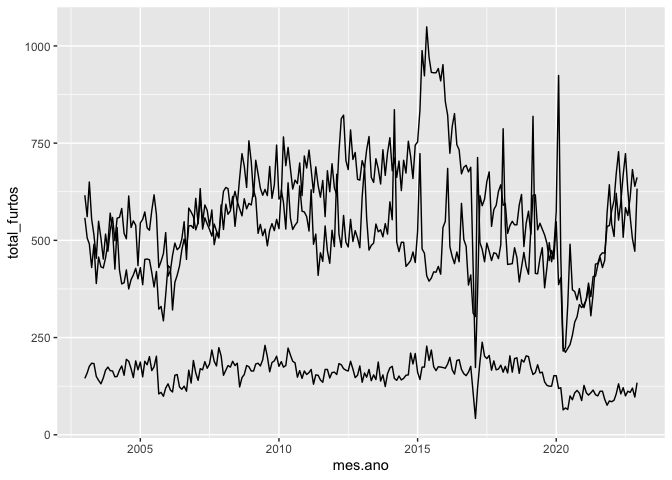
\includegraphics[keepaspectratio]{Aula6_files/figure-latex/evolucao furtos base 1-1.pdf}}

\begin{enumerate}
\def\labelenumi{\arabic{enumi}.}
\setcounter{enumi}{1}
\tightlist
\item
  Apenas fornecer a base para o ggplot e deixar toda a parametrização
  para o elemento geométrico
\end{enumerate}

\begin{Shaded}
\begin{Highlighting}[]
\FunctionTok{ggplot}\NormalTok{(}\AttributeTok{data =}\NormalTok{ crimes.regioes) }\SpecialCharTok{+} \FunctionTok{geom\_line}\NormalTok{(}\FunctionTok{aes}\NormalTok{(}\AttributeTok{x =}\NormalTok{ mes.ano, }\AttributeTok{y =}\NormalTok{ total\_furtos, }\AttributeTok{group =}\NormalTok{ AISP))}
\end{Highlighting}
\end{Shaded}

\pandocbounded{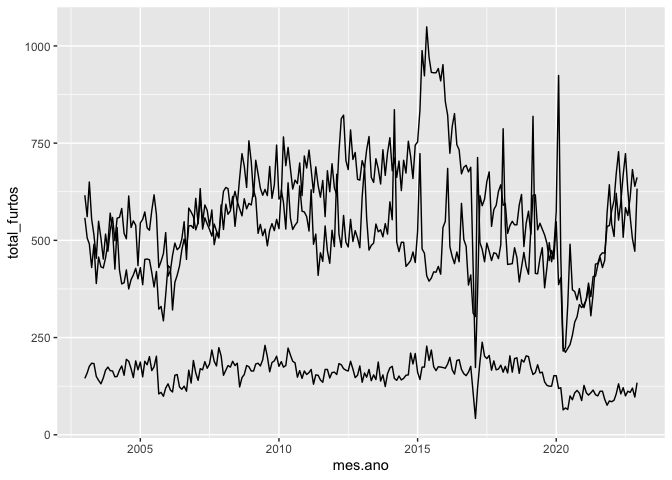
\includegraphics[keepaspectratio]{Aula6_files/figure-latex/evolucao furtos base 2-1.pdf}}
\#\# Adicionando cores ao gráfico

\begin{Shaded}
\begin{Highlighting}[]
\FunctionTok{ggplot}\NormalTok{(}\AttributeTok{data =}\NormalTok{ crimes.regioes, }\FunctionTok{aes}\NormalTok{(}\AttributeTok{x =}\NormalTok{ mes.ano, }\AttributeTok{y =}\NormalTok{ total\_furtos, }\AttributeTok{group =}\NormalTok{ AISP, }\AttributeTok{color =}\NormalTok{ aisp.nm)) }\SpecialCharTok{+} 
  \FunctionTok{geom\_line}\NormalTok{()}
\end{Highlighting}
\end{Shaded}

\pandocbounded{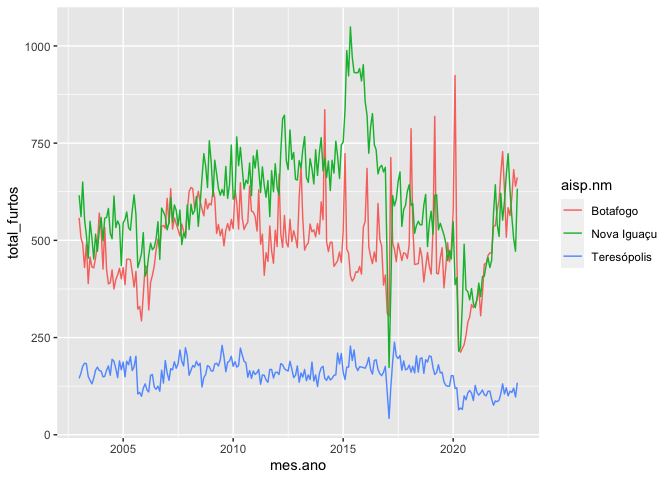
\includegraphics[keepaspectratio]{Aula6_files/figure-latex/evolucao furtos base 1 com cores-1.pdf}}

\subsection{Alterando o tema gráfico}\label{alterando-o-tema-gruxe1fico}

\begin{Shaded}
\begin{Highlighting}[]
\FunctionTok{ggplot}\NormalTok{(}\AttributeTok{data =}\NormalTok{ crimes.regioes, }\FunctionTok{aes}\NormalTok{(}\AttributeTok{x =}\NormalTok{ mes.ano, }\AttributeTok{y =}\NormalTok{ total\_furtos, }\AttributeTok{group =}\NormalTok{ AISP, }\AttributeTok{color =}\NormalTok{ aisp.nm)) }\SpecialCharTok{+} 
  \FunctionTok{geom\_line}\NormalTok{() }\SpecialCharTok{+}
  \FunctionTok{theme\_bw}\NormalTok{()}
\end{Highlighting}
\end{Shaded}

\pandocbounded{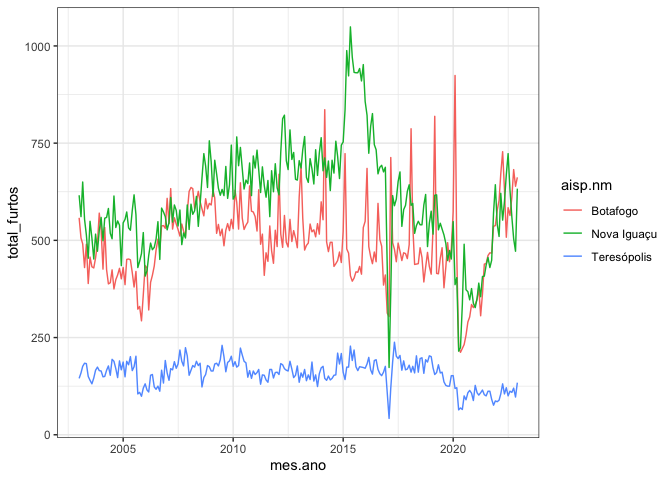
\includegraphics[keepaspectratio]{Aula6_files/figure-latex/evolucao furtos base 1 com cores e com tema-1.pdf}}

\subsection{Ajustando os eixos e títulos do
gráfico}\label{ajustando-os-eixos-e-tuxedtulos-do-gruxe1fico}

\begin{Shaded}
\begin{Highlighting}[]
\FunctionTok{ggplot}\NormalTok{(}\AttributeTok{data =}\NormalTok{ crimes.regioes, }\FunctionTok{aes}\NormalTok{(}\AttributeTok{x =}\NormalTok{ mes.ano, }\AttributeTok{y =}\NormalTok{ total\_furtos, }\AttributeTok{group =}\NormalTok{ AISP, }\AttributeTok{color =}\NormalTok{ aisp.nm)) }\SpecialCharTok{+} 
  \FunctionTok{geom\_line}\NormalTok{() }\SpecialCharTok{+}
  \FunctionTok{xlab}\NormalTok{(}\StringTok{"Período de Análise"}\NormalTok{) }\SpecialCharTok{+}
  \FunctionTok{ylab}\NormalTok{(}\StringTok{"Ocorrências de roubo registradas"}\NormalTok{) }\SpecialCharTok{+}
  \FunctionTok{labs}\NormalTok{(}\AttributeTok{title =} \StringTok{"Séries temporais de furto por região"}\NormalTok{, }\AttributeTok{subtitle =} \StringTok{"Regiões selecionadas no Estado do Rio de Janeiro"}\NormalTok{, }\AttributeTok{caption =} \StringTok{"Fonte: Instituto de Segurança Pública {-} RJ"}\NormalTok{) }\SpecialCharTok{+}
  \FunctionTok{theme\_bw}\NormalTok{() }\SpecialCharTok{+}
  \FunctionTok{guides}\NormalTok{(}\AttributeTok{colour =} \FunctionTok{guide\_legend}\NormalTok{(}\AttributeTok{title =} \StringTok{"Regiões de Segurança Pública"}\NormalTok{))}
\end{Highlighting}
\end{Shaded}

\pandocbounded{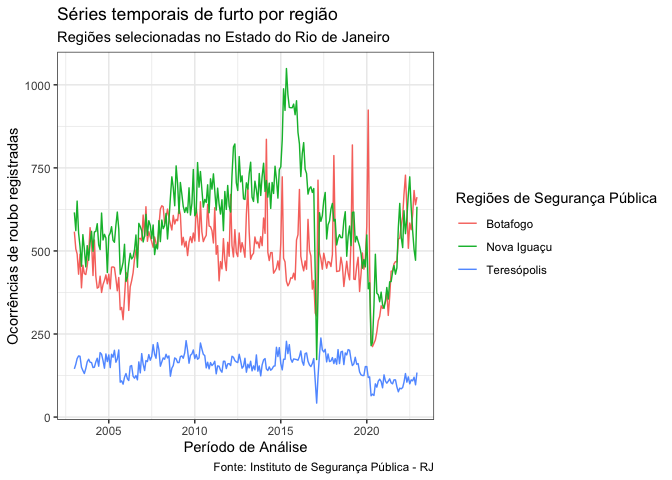
\includegraphics[keepaspectratio]{Aula6_files/figure-latex/evolucao furtos base 1 com cores, com tema e titulos ajustados-1.pdf}}

\subsection{Dever de casa}\label{dever-de-casa}

\begin{Shaded}
\begin{Highlighting}[]
\FunctionTok{ggplot}\NormalTok{(}\AttributeTok{data =}\NormalTok{ crimes.regioes, }\FunctionTok{aes}\NormalTok{(}\AttributeTok{x =}\NormalTok{ mes.ano, }\AttributeTok{y =}\NormalTok{ total\_furtos, }\AttributeTok{group =}\NormalTok{ AISP, }\AttributeTok{color =}\NormalTok{ furto\_transeunte, }\AttributeTok{shape =}\NormalTok{ aisp.nm)) }\SpecialCharTok{+} 
\FunctionTok{geom\_line}\NormalTok{() }\SpecialCharTok{+} 
\FunctionTok{geom\_point}\NormalTok{() }\SpecialCharTok{+}
\FunctionTok{xlab}\NormalTok{(}\StringTok{"Período de Análise"}\NormalTok{) }\SpecialCharTok{+}
\FunctionTok{ylab}\NormalTok{(}\StringTok{"Ocorrências de roubo registradas"}\NormalTok{) }\SpecialCharTok{+}
\FunctionTok{labs}\NormalTok{(}\AttributeTok{title =} \StringTok{"Séries temporais de furto por região"}\NormalTok{, }\AttributeTok{subtitle =} \StringTok{"Regiões selecionadas no Estado do Rio de Janeiro"}\NormalTok{, }\AttributeTok{caption =} \StringTok{"Fonte: Instituto de Segurança Pública {-} RJ"}\NormalTok{) }\SpecialCharTok{+}
\FunctionTok{theme\_bw}\NormalTok{() }\SpecialCharTok{+}
\FunctionTok{scale\_colour\_gradient}\NormalTok{(}\AttributeTok{low =} \StringTok{"yellow"}\NormalTok{, }\AttributeTok{high =} \StringTok{"red"}\NormalTok{, }\AttributeTok{na.value =} \ConstantTok{NA}\NormalTok{) }\SpecialCharTok{+}
\FunctionTok{guides}\NormalTok{(}\AttributeTok{colour =} \FunctionTok{guide\_colourbar}\NormalTok{(}\AttributeTok{title =} \StringTok{"Furto à traseunte"}\NormalTok{), }\AttributeTok{shape =} \FunctionTok{guide\_legend}\NormalTok{(}\AttributeTok{title =} \StringTok{"Regiões de Segurança Pública"}\NormalTok{))}
\end{Highlighting}
\end{Shaded}

\pandocbounded{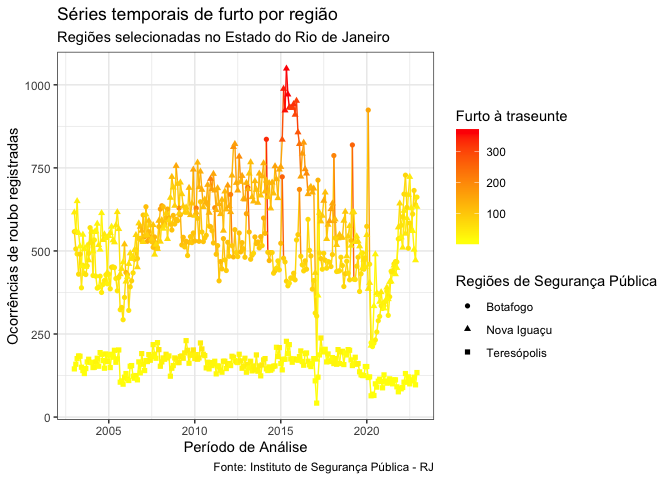
\includegraphics[keepaspectratio]{Aula6_files/figure-latex/evolucao furtos base 1 com cores, com tema e titulos ajustados e variavels adicional-1.pdf}}

\end{document}
